\section{Unterschiedliche Charakter}
Spiele verwenden die unterschiedlichsten Charaktere, nicht nur das Aussehen sondern auch die Komplexität der Körperteile und die Anzahl der Knochen variiert. Um den Charaktercontroller vielseitig einsetzbar zu gestalten wird in diesem Kapitel die Walker Demo Komponenten angepasst um den Einrichtungsprozess zu vereinfachen und unterschiedliche Charakter Körperstrukturen zu erlauben. Es wird der Einrichtungsprozess am Beispiel eines Mixamo 3D Charakter Modells dargestellt. Anschließend werden mit der Mixamo Charakter trainiert und das Ergebnis analysiert. Abschließend werden Verbesserungsansätze für aufgetretene Probleme behandelt.

Der ausgewählte Charakter ist der Y Bot Charakter welcher in Abbildung \ref{fig:charakter_mixamo} zu sehen ist. Der Y Bot besteht ausgenommen der Finger und Zehen aus 22 Knochen. Um das Training zu beschleunigen werden für alle Versuche die Zehen als Vorderfuß und die Finger mit dem Handknochen zusammengefaßt.

\begin{figure}[H]
  \centering  
  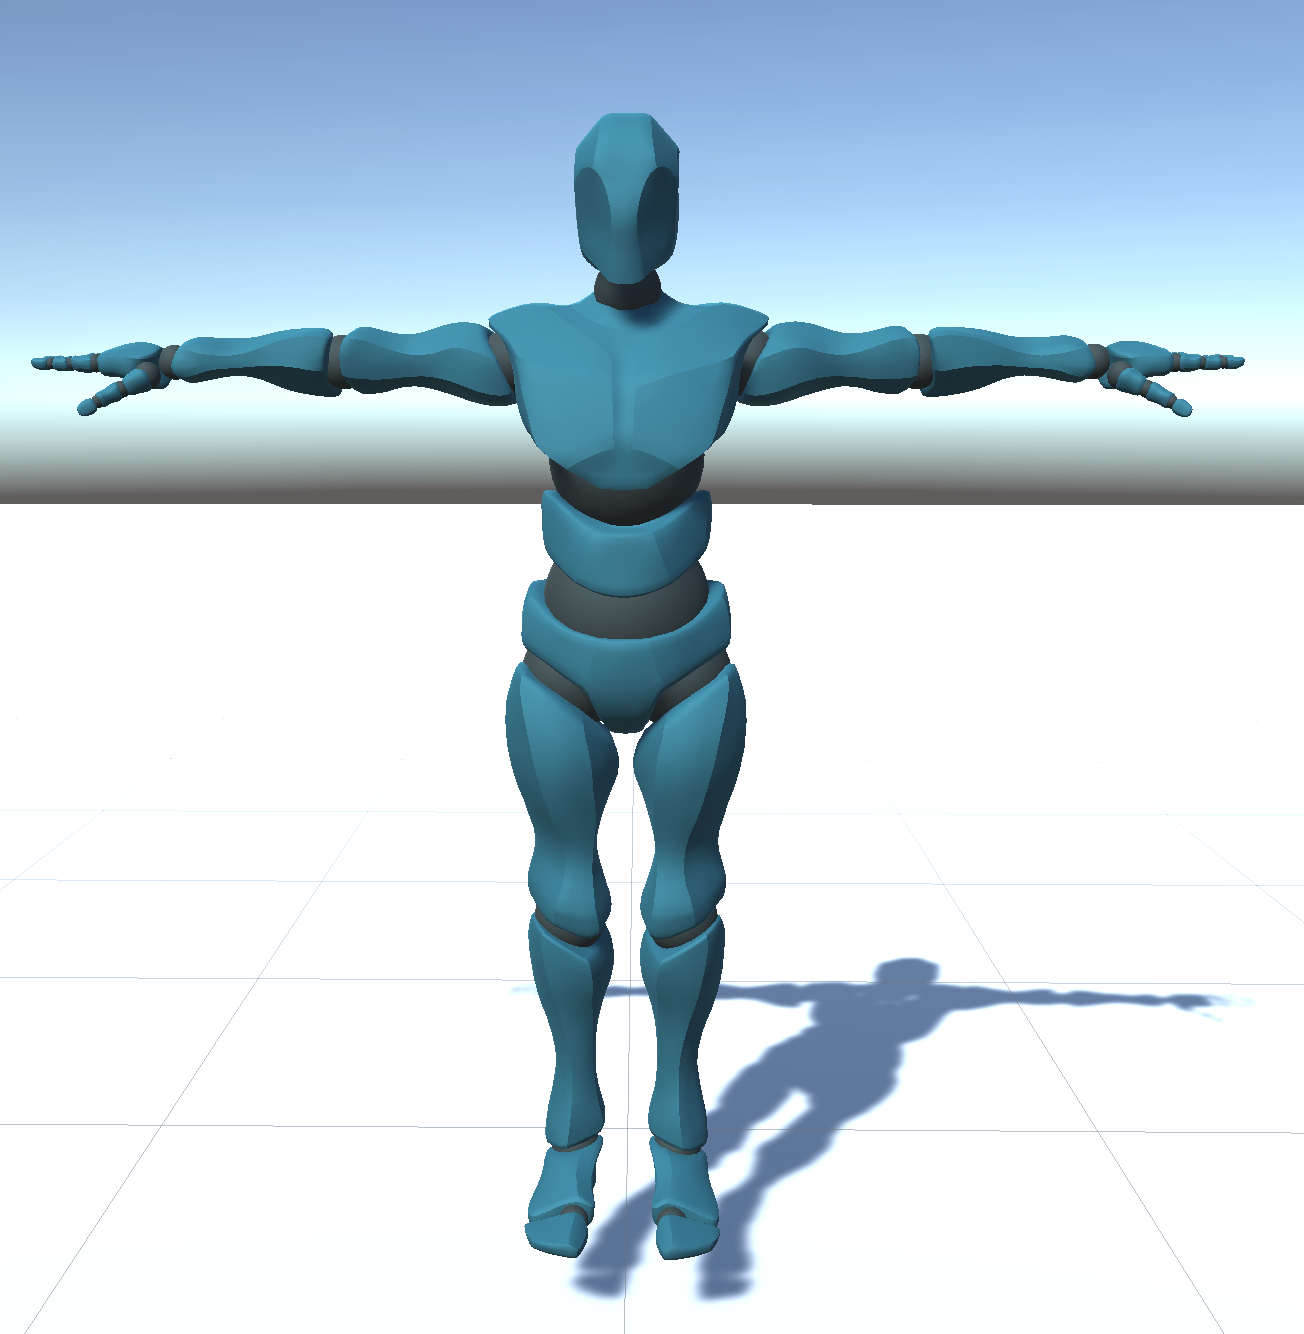
\includegraphics[scale=0.5]{img/charakter_mixamo}
  \caption{Mixamo Charakter Y Bot}
  \label{fig:charakter_mixamo}
\end{figure}

\subsection{Anpassungen}

\subsection{Einrichtung}



Als erstes muss für jedes Körperteile eine passende Kollisionskomponenten ausgewählt und die Größe angepasst werden. Anschließend muss jedes Körperteil eine Festkörperkomponente erhalten. Anschließend müssen die Festkörper- und Gelenkkomponenten hinzugefügt und konfiguriert werden. Die Gewichte der Körperteile wurden im ersten Versuch von der Walker Demo übernommen. Gleichermaßen wurden die Winkellimits für die Gelenke übernommen. Die zusätzlichen Körperteile wurden vereinfacht. Der Oberkörper besteht im Mixamo Modell aus den Schulterknochen sowie dem obersten Wirbel der Wirbelsäule. Die Wirbelsäule besteht im Mixamo Modell aus 2 Wirbeln anstatt dem einen Wirbel des Läufers aus der Demo. Zuletzt sind die Füße noch in Fuß und Vorderfuß aufgeteilt. Bei diesen Änderungen der Körperstruktur wurden die Gewichte und Winkellimits des vereinfachten Körpers auf die komplexeren Körperstrukturen aufgeteilt.

\begin{table}[H]
  \centering
  {\rowcolors{1}{gray!10}{white}
  \begin{tabular}{ |p{3cm}|p{3cm}|p{2cm}|p{4cm}|p{2cm}| }
  \hline
  \textbf{Körpertei}l& \textbf{Verbundenes Körperteil} & \textbf{Gewicht} & \textbf{Winkellimits} & \textbf{Form} \\
  \hline
  Hüfte & - & 15kg & - & Kapsel \\
  \hline
  Wirbel 1 & Hüfte & 6kg & x(-20,20) y(-20,20) z(-15,15) & Kugel \\
  \hline
  Wirbel 2 & Wirbel 1 & 4kg & - & Kugel \\
  \hline
  Wirbel 3 & Wirbel 2 & 3kg & x(-20,20) y(-20,20) z(-15,15) & Kugel \\
  \hline
  Schulter LR & Wirbel 2 & je 2kg& - & Kugel \\
  \hline
  Nacken & Wirbel 3 & 1kg & - & Kugel \\
  \hline
  Kopf & Nacken & 6kg & x(-30,10) y(-20,20) & Kapsel \\
  \hline
  Oberarm LR & Oberkörper & je 4kg & x(-60,120) y(-100,100) & Kapsel \\
  \hline
  Unterarm LR & Oberarm & je 3kg & x(0,160) & Kapsel \\
  \hline
  Hand LR & Unterarm & je 2kg & - & Quader \\
  \hline
  Oberschenkel LR & Hüfte & je 14kg& x(-90,60) y(-40,40) & Kapsel \\
  \hline
  Unterschenkel LR & Oberschenkel & je 7kg &  x(0,120) & Kapsel \\
  \hline
  Fuß LR & Unterschenkel & je 4kg & x(-20,20) y(-20,20) z(-20,20) & Quader \\
  \hline
  Vorderfuß LR & Fuß & je 1kg & - & Quader \\
  \hline
  \end{tabular}}
  \caption{Mixamo Charakter Körperteile}
  \label{table:mixamo_körperteile}
\end{table}

Anschließend kann jedem Körperteil die Körperteilkomponente hinzugefügt werden. Die Körperteilkomponente (Abbildung \ref{fig:komponente_bodypart}) definiert die Körperteile für den Agenten.
\begin{figure}[H]
  \centering  
  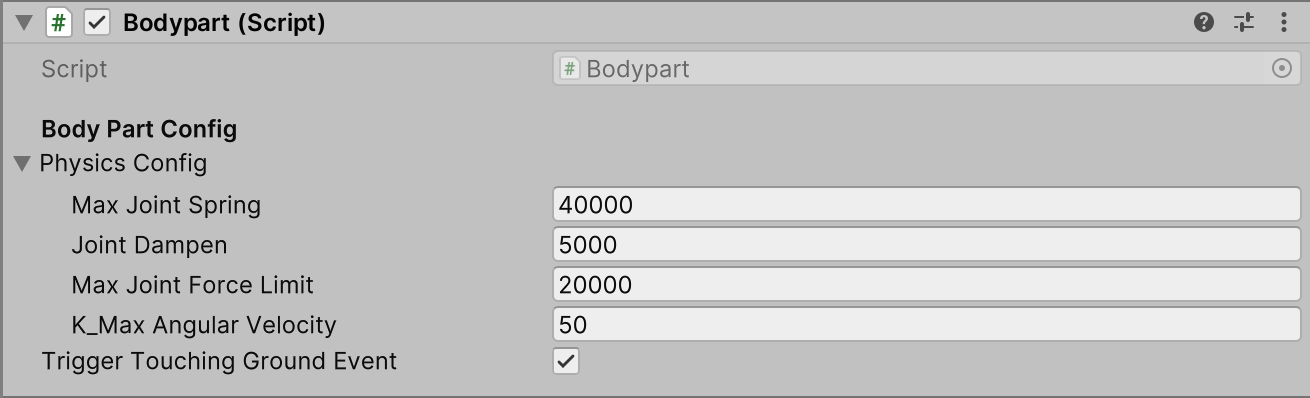
\includegraphics[scale=0.5]{img/komponente_bodypart}
  \caption{Körperteilkomponente}
  \label{fig:komponente_bodypart}
\end{figure}

\begin{itemize}
  \item Physics Config: legt die Kraft des Gelenks und die maximale rotations Geschwindigkeit der Festkörper fest.
  \item Trigger Touching Ground Event: legt fest ob das Körperteil beim berühren des Bodens ein Event auslöst oder nicht
\end{itemize}

Im letzten Schritt muss noch der Walkeragent hinzugefügt und konfiguriert werden.